%# -*- coding: utf-8-unix -*-
%%==================================================
%% chapter03.tex for SJTU Bachelor Thesis
%%==================================================

%\bibliographystyle{sjtu2}%[此处用于每章都生产参考文献]
\chapter{粗粒度的的调度器设计}
\label{chap:LB}
本章讲述如何利用巨型虚拟机设计一个高效的集群调度器,在不影响集群中任务的服务质量的同时,也可以提高集群总体CPU资源的使用率。为此,我们提出三条设计理念(设计目标),再详述我们的设计细节,并且就每条设计目标讨论设计的目的是否达成。
\section{设计理念与设计目标}
本文设计调度器应当均衡地将工作负载分配到各个节点上,从而使集群资源得到最大化的利用,这是所有分布式集群调度器都应当达到的目标。此外,我们设计的调度器应当符合如下三条理念:

\noindent\textbf{调度过程开销较小}\quad 一个高效的集群调度器应当尽量缩短任务负载的迁移时间,同时不影响任务负载对外提供服务的质量,否则调度产生的性能提升将被额外的开销所掩盖。如第二章第四节所述,集群中的调度可以通过三种迁移方式得以实现:进程迁移,容器热迁移,虚拟机热迁移。进程迁移关注的抽象层次较高,涉及到了操作系统中具体数据结构的迁移,例如和其他进程共享的文件、内存等,目前还没有迁移这些数据结构的方法,遇到了残余依赖的问题。容器的热迁移虽然将残余依赖打包在一个容器实例中,但是有较长的下线时间,对容器内的任务有较大影响,故我们不采用容器作为调度器的技术基础。虚拟机为上层软件提供了简易的硬件接口,抽象层次较低,所以虚拟机的热迁移应当是我们关注的重点。虚拟机热迁移的主要问题是,需要迁移的内存是整个客户机操作系统的内存,占用了较大的网络带宽。虽然历史上有一些方法减小带宽,如并行传送\cite{parallelm}、差分压缩\cite{compression}等方式减小虚拟机热迁移所带来的网络开销,但这些方法治标不治本:应当有选择的传输工作负载的状态而非传输整个操作系统的状态。本文应当设计一个减小热迁移中传输内存范围的机制,同时尽可能得减小或消除下线时间。

\noindent\textbf{无需修改现有软件}\quad 数据中心内运行的任务种类多种多样,数目巨大,如果调度器需要现有软件的配合才能实现高效的迁移功能,则这类调度器必然无法得到广泛的应用。所以,应当设计一个与现有操作系统(如Linux)适配的且不影响现有应用程序逻辑的调度方法。进一步的,应该利用现有操作系统的接口和机制,而不是修改现有调度器(如Linux中的完全公平调度器)。故本文中调度器的实现应当不修改Linux内核的逻辑(例如,不使用半虚拟化技术),也不需要现有软件的配合。

\noindent\textbf{动态感知工作负载}\quad 能够动态地根据节点的工作负载作出最合理的迁移决定是本文的重中之重。相比于设计一个作出单次调度决策的调度器,动态感知工作负载的变化情况作出多次调度决策必然能够更加充分地使用资源。有两类方式根据工作负载作出迁移决定:主动式决策(proactive)和被动式决策(reactive)。主动式决策通过对系统的精确采样,主动预测工作负载的变化情况(例如使用机器学习技术建立模型进行训练),作出调度决策。这类方式为了使采集的数据具有很好的代表性,势必会进行更加频繁的采样,造成巨大的开销;其次,工作负载的变化情况本身并不可预知,除了一些运行时间较短的任务有着较为固定的工作负载变化模式,但这些任务对集群整体产生的影响十分有限。故我们选择被动式的决策方式,在系统负载发生改变之后,以最快的速度根据负载情况完成任务调度,即可适应不断变化的工作负载。

\section{粗粒度调度器的设计}
我们受到Barrelfish操作系统设计理念的启发:Barrelfish将操作系统内核状态分割成多个副本,每个副本固定在一个独占的CPU核上,从而避免了基于缓存一致性这一硬件机制的大量核间数据的传输,提高了操作系统的可扩展性。我们将此概念进一步延伸,从而达到我们的目的:虚拟机热迁移所带来的网络开销中含有不必要的操作系统内存的部分,可以将客户机的大部分状态固定在不同的节点上,从而在迁移客户机内部工作负载时,无需传输和工作负载无关的状态,其中包括客户机操作系统的大量数据和代码,以及客户机中其他任务的状态,而只需传输工作负载所拥有的状态(如其频繁访问的内存页)。为达成这个目的,我们需要一个分布式的虚拟机,运行在一个分布式集群上。这样一来,客户机的状态分布在集群的每个节点上,免去了大量内存页的迁移需求。而巨型虚拟机基于现有的单机虚拟机管理器QEMU-KVM,开发年限较长,与现有系统的兼容性良好,且运行稳定,可以运行主流的操作系统,所以我们选择巨型虚拟机实现上述目标。
\subsection{迁移机制概述}
\begin{figure}[!htp]
  \centering
  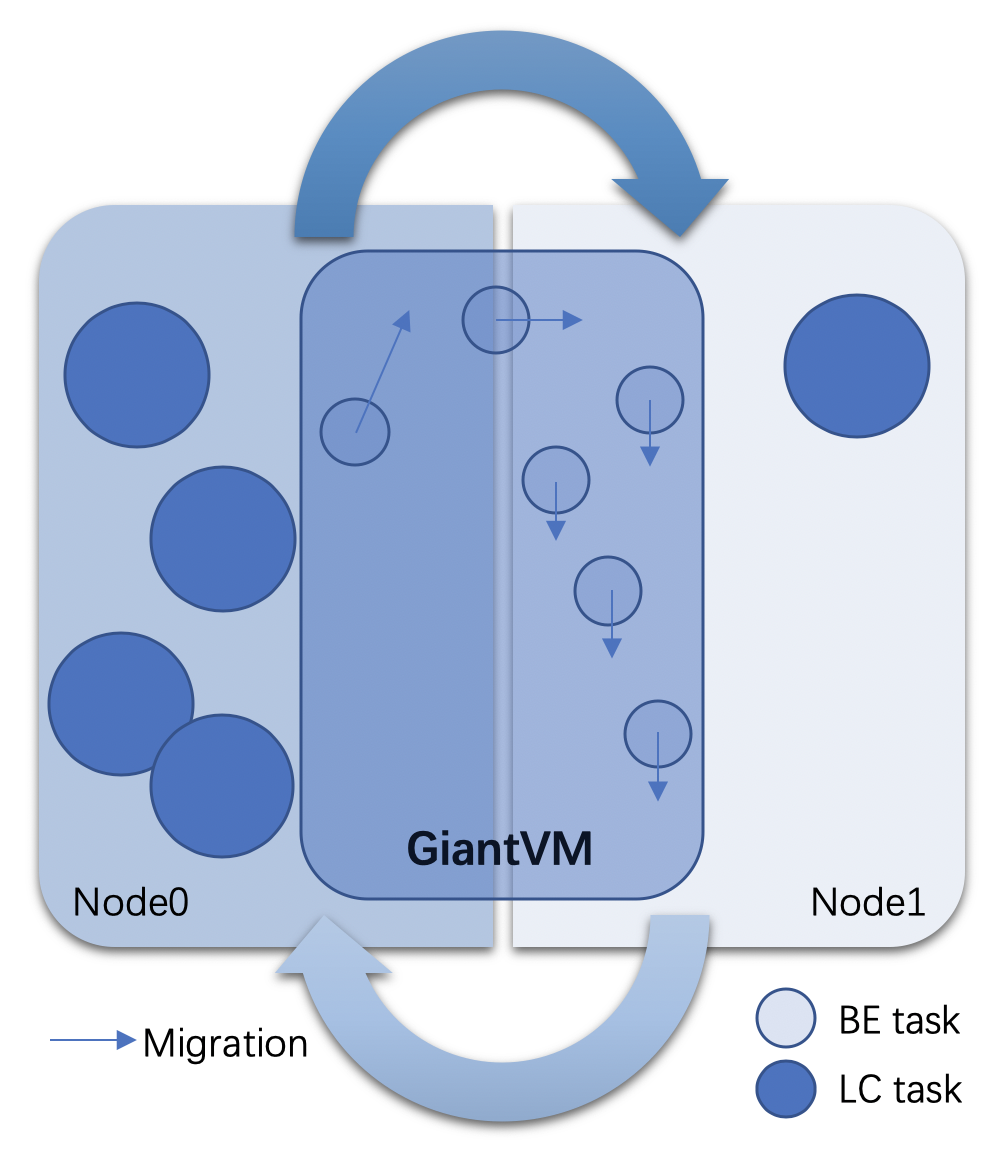
\includegraphics[width=8cm]{schedule.png}
  \bicaption[基于GiantVM的任务迁移机制]
    {基于GiantVM的任务迁移机制}
    {Task Migration Mechanism Based on GiantVM}
  \label{fig:schedule}
\end{figure}

我们将巨型虚拟机的客户机操作系统作为集群节点之间交换任务负载的桥梁:我们把任务分为可迁移任务(migratable tasks)和不可迁移任务(fixed tasks)。在图\ref{fig:schedule}中,颜色较深的圆圈代表不可迁移任务,系统通常为其分配较充足的资源,故用大圆表示,而颜色较浅的小圆代表可迁移任务。巨型虚拟机横跨多个节点,通过分布式虚拟机运输可迁移任务。在每个迁移周期中,我们扫描整个系统内所有的进程,选择一部分可迁移进程加入巨型虚拟机的客户机中。巨型虚拟机对客户机提供一个模拟的NUMA硬件环境,每一个NUMA节点代表分布式集群中的一个节点,从而使得客户机得知底层的硬件环境的拓扑结构。我们在客户机中设计一个专用的调度器,它可以动态感知每个NUMA节点下的真实物理节点的负载。当迁移条件满足时(如宿主集群某个节点CPU占用率超过阈值),调度器读取每个节点的负载,选取负载最低的节点,将可迁移任务调度到该NUMA节点上。被迁移的任务虽然不会有下线时间,但是由于分布式共享内存组件的存在,需要对一部分内存页进行迁移,也会造成一定的性能影响。借助于巨型虚拟机,任务的迁移过程有所变化:客户机中的进程向运行在其他NUMA节点的vCPU上迁移等同于进程在集群节点间迁移。如图\ref{fig:schedule}所示,Node0中不可迁移型任务对系统资源占用过高,于是触发了可迁移型任务在巨型虚拟机中的迁移。

对于如何将任务分类为可迁移任务和不可迁移任务,目前的实现是把延迟敏感型任务(LC tasks)作为不可迁移任务,它们不能承受性能的损失(例如一些业务进程,如果延迟提高则会使得收益受到影响),而将尽力而为型任务(BE tasks)作为可迁移任务,其延迟增长对用户的影响不大(例如一些用于开发实验的进程,为了测试未投入使用的代码,或一些数据分析程序)。在图\ref{fig:schedule}中LC型任务即不可迁移任务,BE型任务即可迁移任务。在这样的分类之下,延迟敏感型任务的服务质量将不会受到影响,而尽力而为型任务正好将延迟敏感型任务未使用的资源利用起来:由于延迟敏感型任务无法承受性能损失,系统为其分配了足够多的CPU资源,来应对其可能出现的CPU利用率突增,而事实上大部分时间内这些CPU资源都无法完全利用,于是当延迟敏感型任务占用较低时,巨型虚拟机将尽力而为型任务调度到对应的节点上,填补CPU使用率的空缺,从而提高了集群总体的CPU资源占用率。

\subsection{调度脚本实现}
\begin{figure}[!htp]
  \centering
  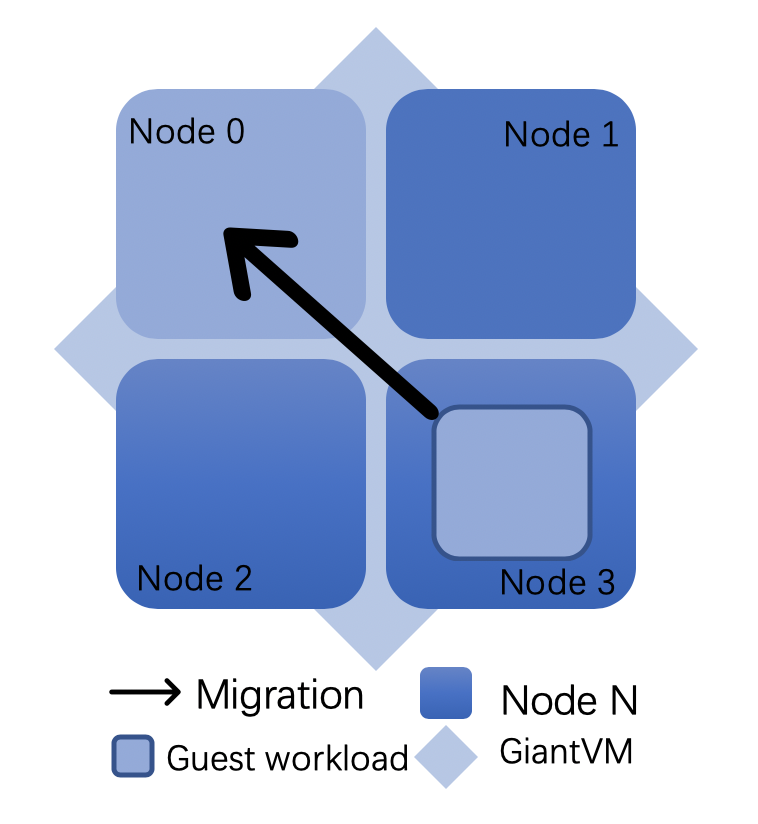
\includegraphics[width=6cm]{coarse.png}
  \bicaption[基于巨型虚拟机的粗粒度的调度]
    {基于巨型虚拟机的粗粒度的调度过程}
    {Coarse Grained Scheduling Based on GiantVM}}
  \label{fig:coarse}
\end{figure}

\begin{algorithm}[h]
\begin{algorithmic}[ruled,1]
\Function {set\_affinity\_all}{$node\_cpu\_list$}
\For{each $task, irq, wq\in OS$}
\State
\Call{set\_affinity}{$task, node\_cpu\_list$}
\State
\Call{set\_affinity}{$irq, node\_cpu\_list$}
\State
\Call{set\_affinity}{$wq, node\_cpu\_list$}
\EndFor
\EndFunction
\State
\State
\Call {set\_affinity\_all}{$node0\_cpu\_list$}
\State
\While{true}
\State
\Call {sleep}{$INTERVAL$}
\State $min\_stealtime,\,min\_stealtime\_node \gets find\_min\_stealtime\_node()$
\If {$this\_node &= &= min\_stealtime\_node \lor this\_node\_stealtime < threshold$}
\State $continue$
\EndIf
\State $cpu\_list \gets get\_cpu\_list(min\_stealtime\_node)$
\State
\Call {set\_affinity\_all} {$cpu\_list$}
\EndWhile
\end{algorithmic}
\caption{粗粒度进程调度算法}
\label{algo:coarse}
\end{algorithm}
事实上,上节所述的调度机制应当使用C代码来实现,即在Linux内核中添加一个新的调度器类(Linux内核中有多种调度算法,每种调度算法自成一个调度器类,由核心调度器调用。现有的调度类有完全公平调度类、实时调度类、空闲调度类)。然而操作系统已经给用户层提供了足够多的接口来实现我们所说的调度策略,而增添一个新的调度器类工作量较大,调试各类参数比较困难,故我们选择使用shell脚本实现调度算法。目前在Linux上实现了一个粗粒度调度算法,而细粒度调度算法将作为未来的工作。

对于粗粒度的调度算法,如图\ref{fig:coarse},我们通常将巨型虚拟机部署在四个节点上,只需要找到四个NUMA节点中宿主机占用最低的节点,将客户机中所有的任务迁移到该NUMA节点上即可(颜色深的节点代表其负载较高)。客户机中调度脚本的实现如算法\ref{algo:coarse}所示,对应的bash脚本是rebalance.sh。我们设置rebalance.sh作为系统启动项,系统启动时,调用$set\_affinity\_all()$使得OS中所有的进程都运行在Node0上,Node之间无需做网络通信,缩短了启动时间。此后,每个调度周期中,读取两次累计的steal time做差得到该时段内的steal time,如果当前所有进程运行的节点的steal time超过了一个阈值(50个节拍),即触发迁移,调用$set\_affinity\_all()$将所有进程固定在steal time最低的节点上。虽然这样减少了客户机中进程可以使用的虚拟CPU个数,但是最大程度的减少了网络的开销,由于任何两个NUMA节点之间无需共享内存数据,而只有一个NUMA节点上有任务在运行。

/proc文件夹是Linux内核为用户态程序提供内核信息的文件夹,用户态程序也可通过写入/proc文件夹中的某个文件更改内核的配置。在本文中,我们读取/proc/stat文件的内容完成两个功能:一是获取宿主机节点上的CPU使用率,二是在客户机操作系统中获取steal time。/proc/stat文件包含了自系统启动以来累计的CPU节拍数,CPU空闲的节拍数,以及因为虚拟化所产生的累计的steal time。steal time指虚拟CPU等待物理CPU执行其他宿主机指令或者其他虚拟CPU的时间,直接向客户机反映了宿主机的工作负载状态。这样客户机的运行将被该脚本所控制。进程调度通过taskset指令实现,其本质是修改了task\_struct中的cpumask,即修改了进程可以运行的CPU列表。同时为了最小化NUMA节点之间的内存共享,我们将中断全部发送给该选中的NUMA节点的CPU上(通过写入/proc/irq文件),也将所有workqueue固定在这些CPU上。

\subsection{性能优势}
巨型虚拟机的进程调度等价于虚拟机热迁移,且迁移开销较低,没有下线时间,比较适合资源重分配的集群负载平衡方式(见第\ref{chap:reallocation}节,资源重分配同步于系统中频繁变化的负载,迁移的频率较高)。当巨型虚拟机中的进程被taskset到某一节点上时,由于分布式共享内存模块的内存同步协议,会产生大量的EPT缺页异常,会使得被迁移任务的服务质量严重下降。发生EPT缺页异常后,分布式共享内存模块开始传输该进程的页,直到该进程频繁访问的页被完全传输到目标节点。虽然巨型虚拟机的进程调度会经历如此的性能下降,但是其开销还是远小于虚拟机热迁移的开销,因为分布式共享内存只会在各个节点之间传输被频繁修改的页。根据第\ref{chap:mem}节对于进程虚拟内存空间分布的分析,我们以客户机的物理页为中心讨论巨型虚拟机相比于虚拟机热迁移无需传输哪些页(EPT将客户机物理页映射到宿主机物理页,故讨论客户机物理页即是讨论宿主机物理):(1)所有被客户机内进程映射为只读的客户机物理页,包括内核态和用户态的.text 段和.rodata段。(2)未被映射进入任何客户机进程的虚拟地址空间以及内核虚拟地址空间的物理页。(3)Linux进程有一个当前进程频繁访问的物理页面的集合。由于数据访问的局部性(data/space locality),进程通常有一个固定大小频繁访问的内存区域,故客户机有部分物理内存虽然被映射进入某个虚拟地址空间,但进程很少访问它们。以上三类页面是虚拟机热迁移过程中无法区分的,在迁移一个完整的虚拟机时,必须将其所有使用的宿主机物理页面全部进行迁移。

\section{本章小结}
本章提出了三个集群调度器的设计理念,并且描述了如何使用巨型虚拟机完成集群调度功能,以及其shell脚本实现的粗粒度进程调度算法,动态感知负载情况。本章设计的shell脚本的实现可以在任何Linux操作系统中部署,无需修改现有软件,并且相比于虚拟机热迁移大大缩减了被迁移的页面数量,有较高的迁移性能,且无下线时间,达到了本章开始设定的设计目标。